\documentclass[border=2pt]{standalone}

% Drawing 
\usepackage{tikz}
\usetikzlibrary{decorations.markings}
\tikzset{annotate/.style 2 args={postaction={decorate,decoration={markings,
mark=at position 0 with {\node[circle,inner sep=1.2pt,draw,fill=white,#1]{};},
mark=at position 0.52 with {\arrow[>=stealth,line width=1.5pt]{>};
\node at (0,0.4) {#2};}}}}}

% Notation
\usepackage{physics}
\usepackage{amsmath}

\begin{document}

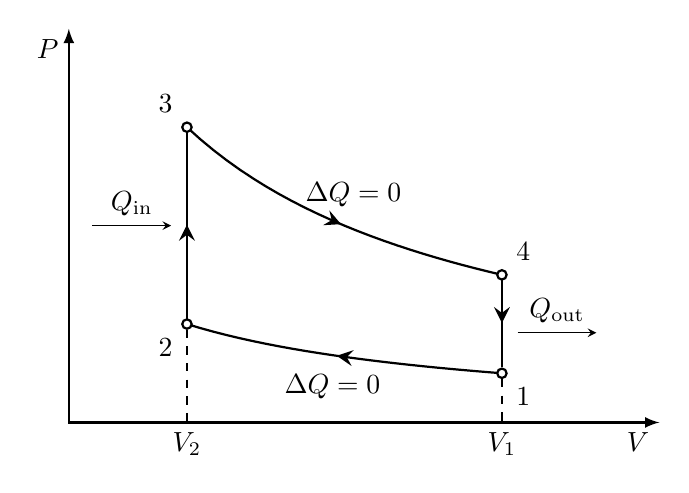
\begin{tikzpicture}
	% Axis
	\draw[latex-latex, thick] (-0.5,5) node[below left]{$P$} |- (7,0) node[below left]{$V$};
	
	\begin{scope}[thick]
	\draw[annotate={label=below right:1,alias=1}{$\Delta Q=0$}] plot[variable=\x,domain=5:1] (\x,{5/(\x+3)});
	\draw[annotate={label=above left:3,alias=3}{$\Delta Q=0$}] plot[variable=\x,domain=1:5] (\x,{15/(\x+3)});
	\draw[annotate={label=below left:2,alias=2}{}] (1,5/4) -- (3);
	\draw[annotate={label=above right:4,alias=4}{}] (5,15/8) -- (1);  
	\end{scope} 
	
	\path (2) -- (3) coordinate[pos=0.5] (23) (1) -- (4) coordinate[pos=0.4] (14);
	
	\draw[stealth-] ([xshift=-2mm]23) -- ++ (-1,0) node[midway,above]{$Q_\text{in}$};
	\draw[-stealth] ([xshift=2mm]14) -- ++ (1,0) node[midway,above]{$Q_\text{out}$};
	
	\draw[dashed, thick] (1) -- (1|-0,0) node[below] {$V_1$};
	\draw[dashed, thick] (2) -- (2|-0,0) node[below] {$V_2$};
	
	% \foreach \i in {0,...,6}
	% {
	% 	\node at (\i,0) {\i};
	% 	\node at (0,\i) {\i};
	% }
\end{tikzpicture}

\end{document}
